
%%% Local Variables:
%%% mode: latex
%%% TeX-master: t
%%% End:

\section{再认识与展望}

\begin{frame}[t]{加大现有数据的利用率和产品化思维}
\begin{itemize}
\item<1-> 面向业务的数据整合
\item<2-> 查询功能设计与开发
\end{itemize}

\begin{overlayarea}{\textwidth}{\textheight}
  \begin{onlyenv}<1>
\begin{figure}
  \centering
  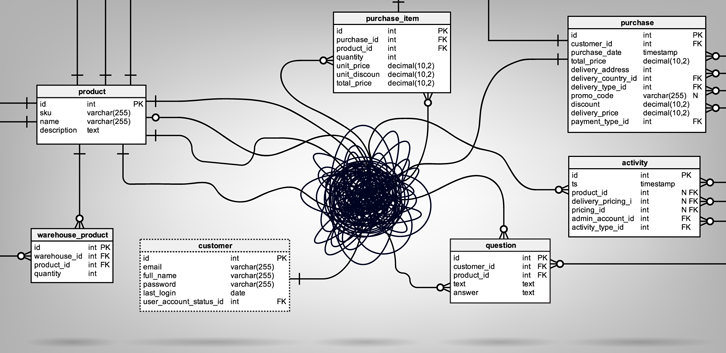
\includegraphics[width=\textwidth]{chp05_传统调查数据整合.png}
  \caption{数据整合要梳理数据结构特征,设计面向业务的数据库对象}
\end{figure}
  \end{onlyenv}

\vspace{-15pt}
  \begin{onlyenv}<2>
\begin{figure}
  \centering
  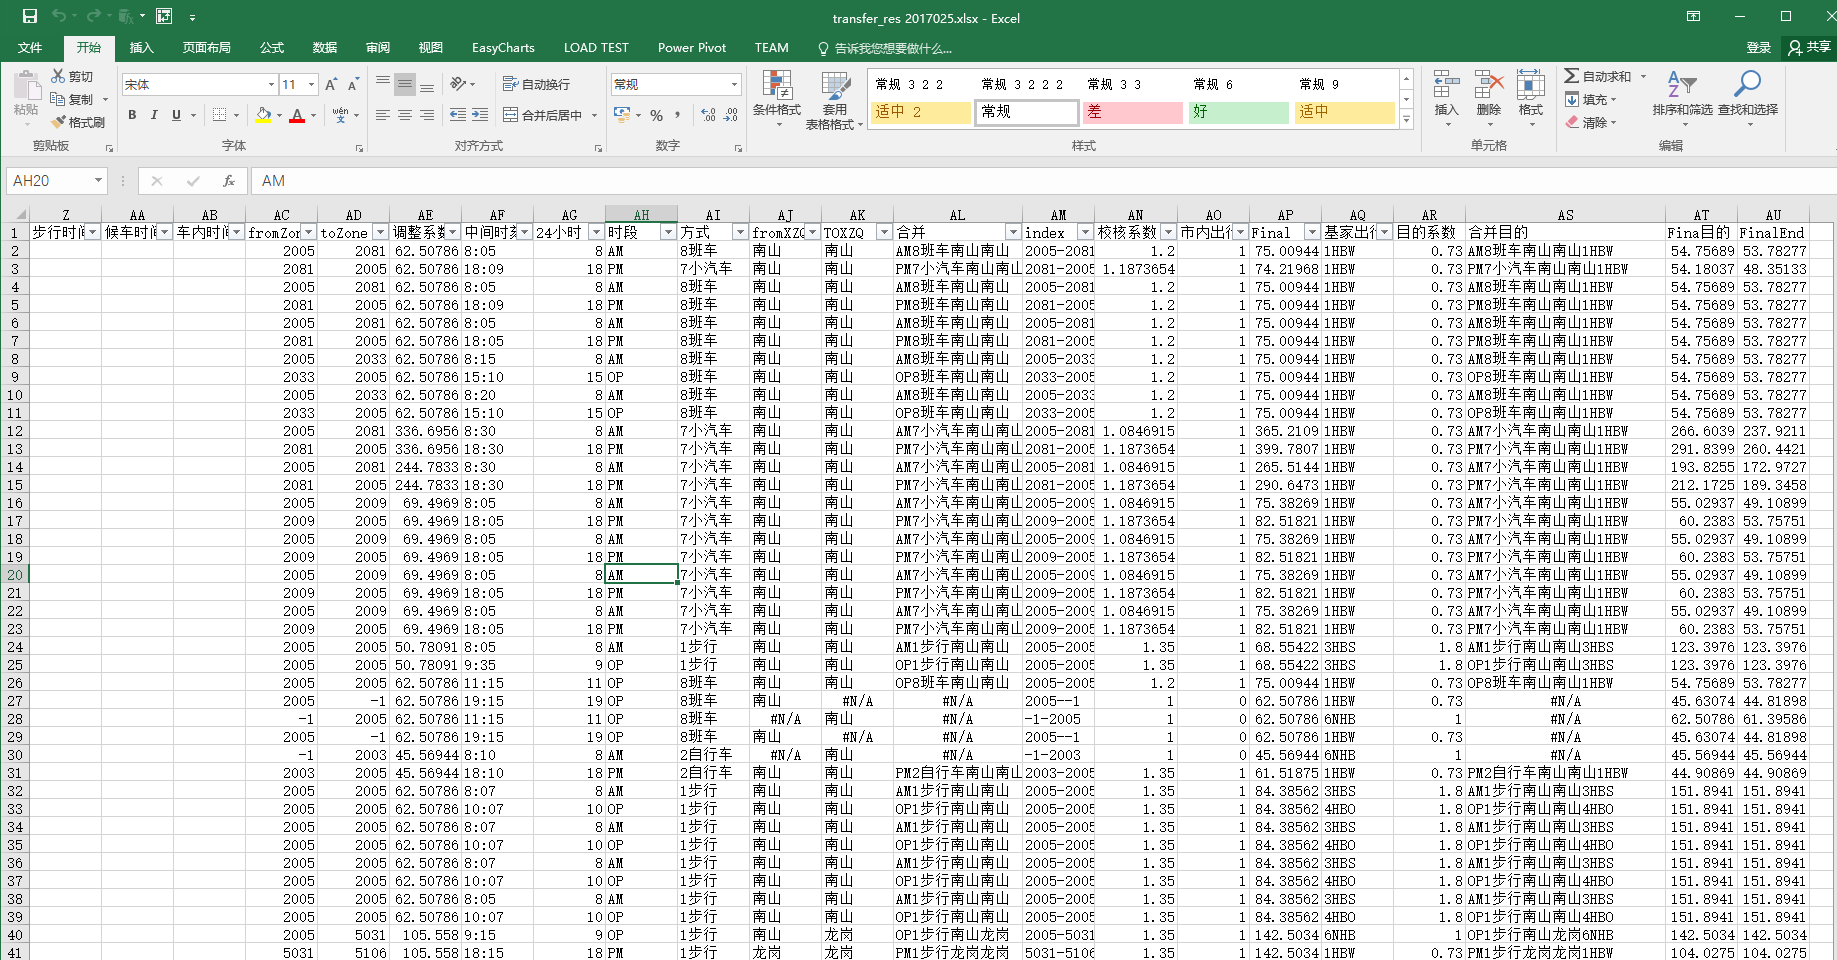
\includegraphics[width=\textwidth]{chp05_excel查询.png}
  \caption{目前还是基于excel进行手动的数据查询分析,没有形成产品化的工具,在日常工作中很难推广和复用}
\end{figure}
  \end{onlyenv}

  \begin{onlyenv}<3>
\begin{figure}
  \centering
  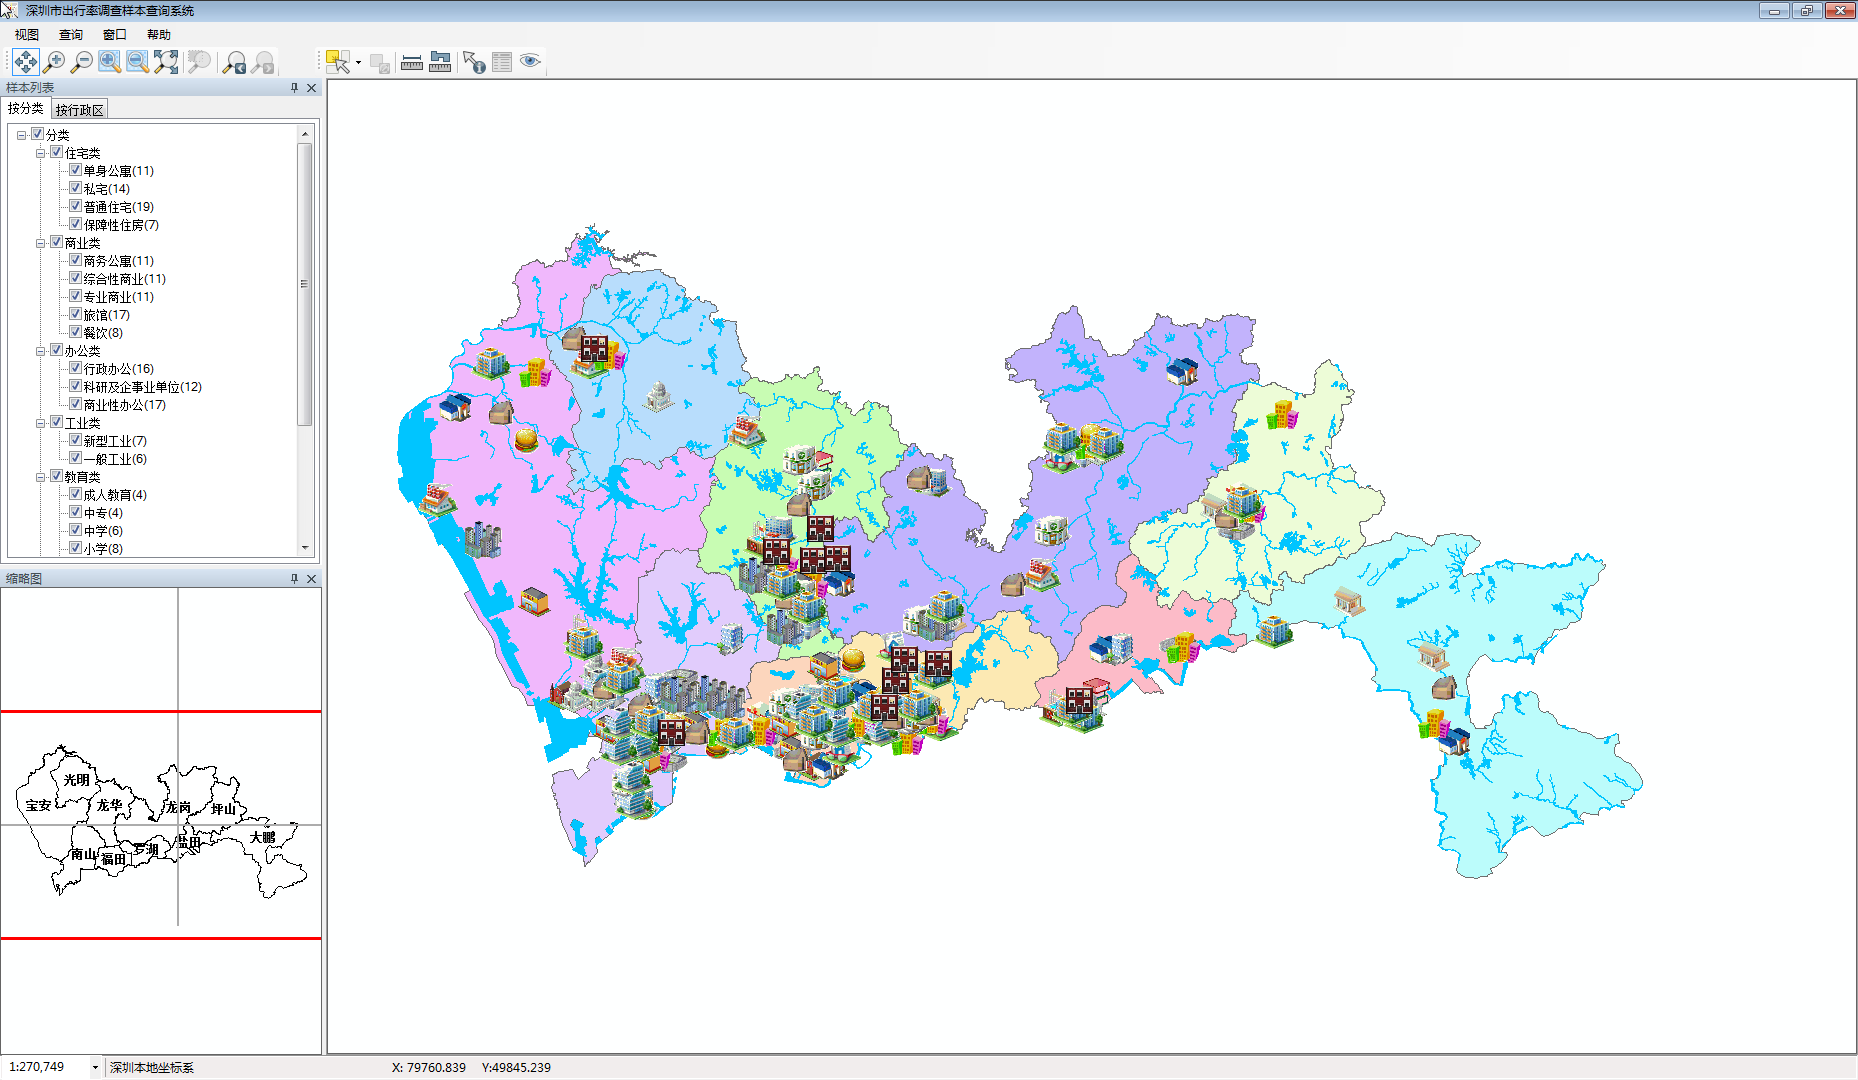
\includegraphics[width=\textwidth]{chp05_数据查询系统.png}
  \caption{基于GIS开发独立的面向业务人员的数据查询系统}
\end{figure}
  \end{onlyenv}

  \begin{onlyenv}<4>
\begin{figure}
  \centering
  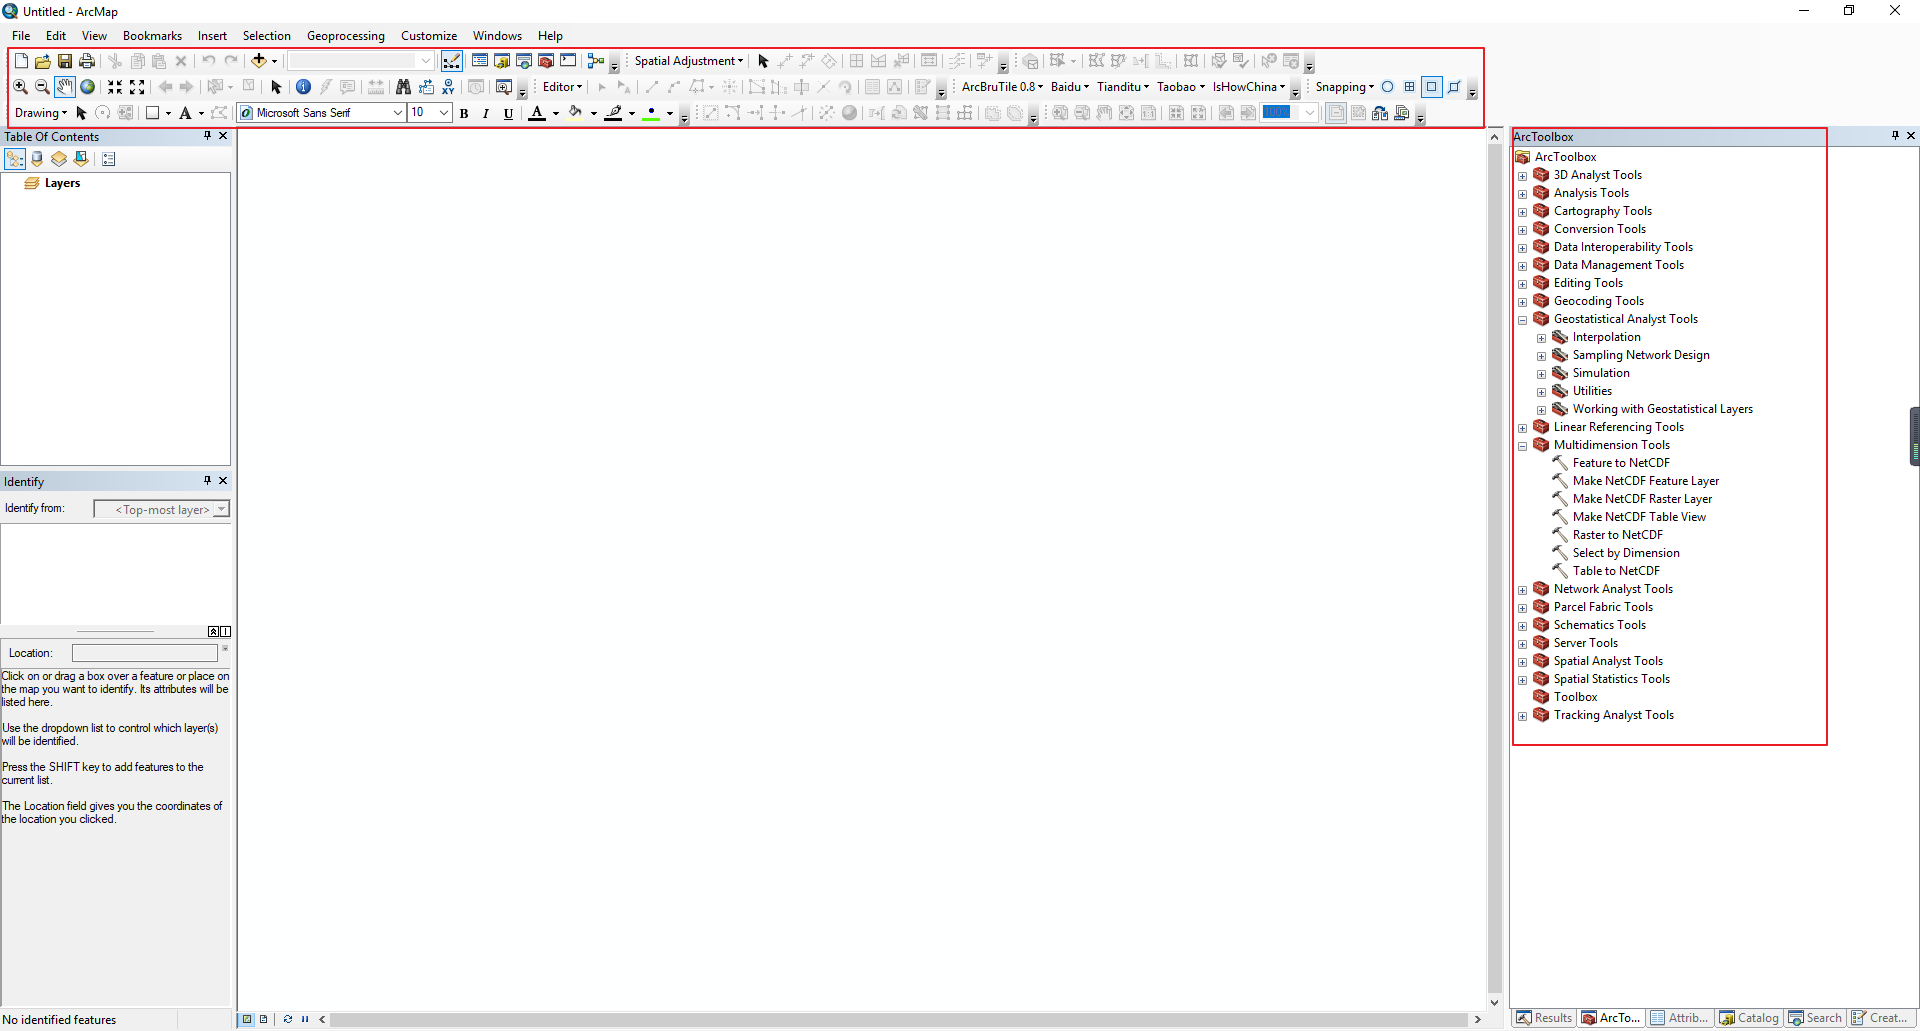
\includegraphics[width=\textwidth]{chp05_查询插件.png}
  \caption{在熟悉的工作平台中以插件的方式实现数据查询}
\end{figure}
  \end{onlyenv}
\end{overlayarea}
\end{frame}

\begin{frame}[t]{提升数据分析的深度}
\begin{itemize}
\item<1-> 现有数据应用主要在传统交通模型和现状的简单指标统计,没有形成分析方法体系,
\emphText{分析程度非常浅}
\item<2-> 交通模型体系在大数据环境下的理论创新,以及空间分析、机器学习等技术手段在交通规划行业的广泛应用
\end{itemize}

\begin{overlayarea}{\textwidth}{\textheight}
  \begin{onlyenv}<1>
\begin{figure}
  \centering
  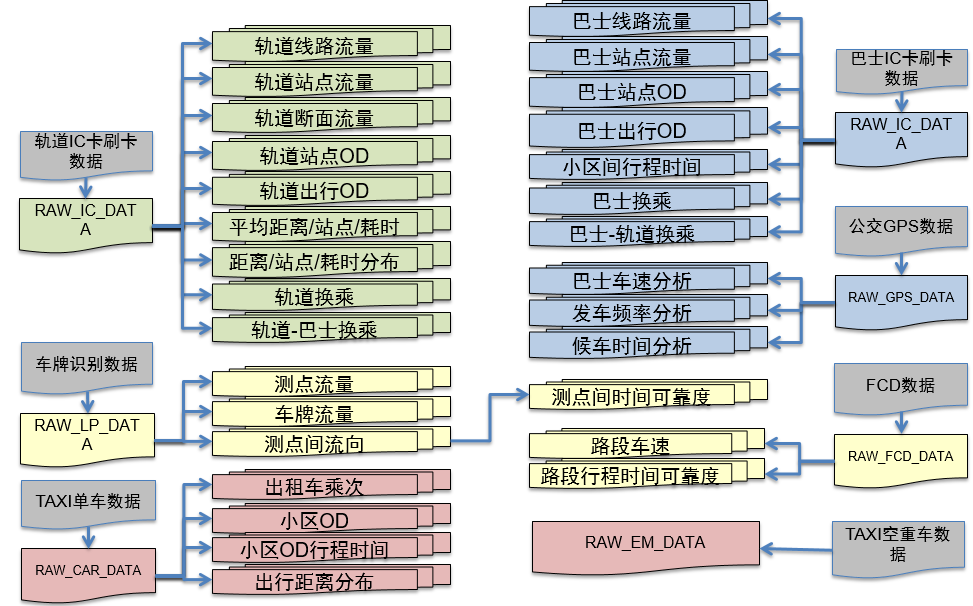
\includegraphics[width=0.75\textwidth]{chp05_简单统计.png}
  \caption{仿真二期系统中同济设计的交通专项统计指标}
\end{figure}
  \end{onlyenv}

\vspace{-15pt}
  \begin{onlyenv}<2>
\begin{figure}
  \centering
  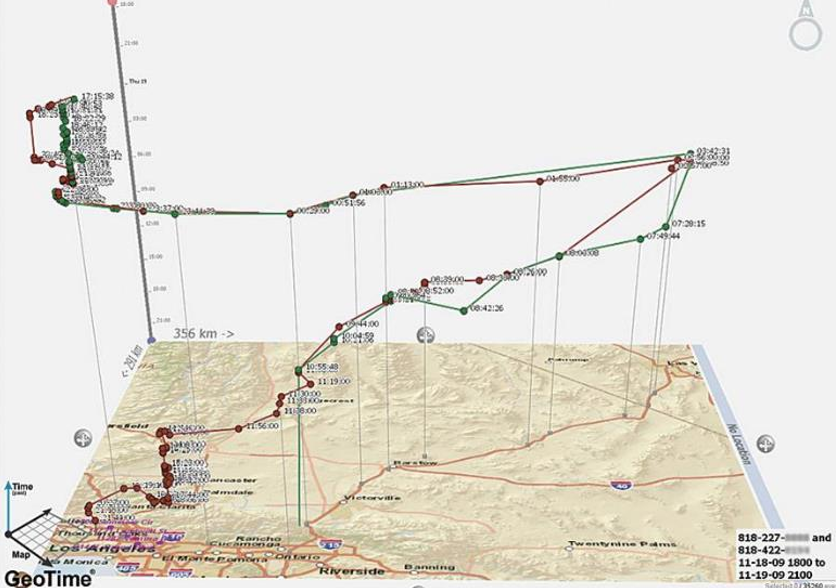
\includegraphics[width=0.7\textwidth]{chp05_geotime.png}
  \caption{交通模型理论的创新}
\end{figure}
  \end{onlyenv}

  \begin{onlyenv}<3>
\begin{figure}
  \centering
  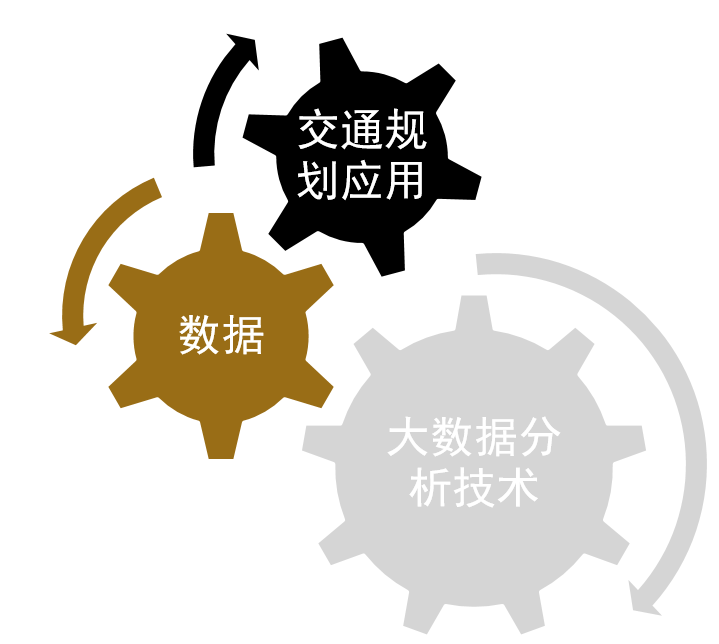
\includegraphics[width=0.55\textwidth]{chp05_大数据业务应用.png}
  \caption{专业的大数据分析手段在行业内的推广普及}
\end{figure}
  \end{onlyenv}
\end{overlayarea}
\end{frame}

\begin{frame}[t]{提升数据分析的深度}
\begin{itemize}
\item 现有数据应用主要在传统交通模型和现状的简单指标统计,没有形成分析方法体系,
\emphText{分析程度非常低下}
\item 交通模型体系在大数据环境下的理论创新,以及空间分析、机器学习等技术手段在交通规划行业的广泛应用
\item<2-> 交通规划业务人员需要提升自身的技术水平,才能够提出具有针对性和可行性和的需求
\end{itemize}
\end{frame}

\begin{frame}[t]{“自下而上”的规划决策}
\begin{itemize}
\item<1-> 数据可以实现规划编制过程中政府、规划师、市民之间的动态互动,实现\emphText{规划调研、方案制定、规划评估、规划实施}等全过程的公众参与
\item<2-> 利用政府开放数据,让公众参与规划过程,可以更加精细化地研究人的行为需求与城市空间的内在关系,体现“以人为本”的规划设计
\end{itemize}

\begin{overlayarea}{\textwidth}{\textheight}
\vspace{-5pt}
  \begin{onlyenv}<1>
\begin{figure}
  \centering
  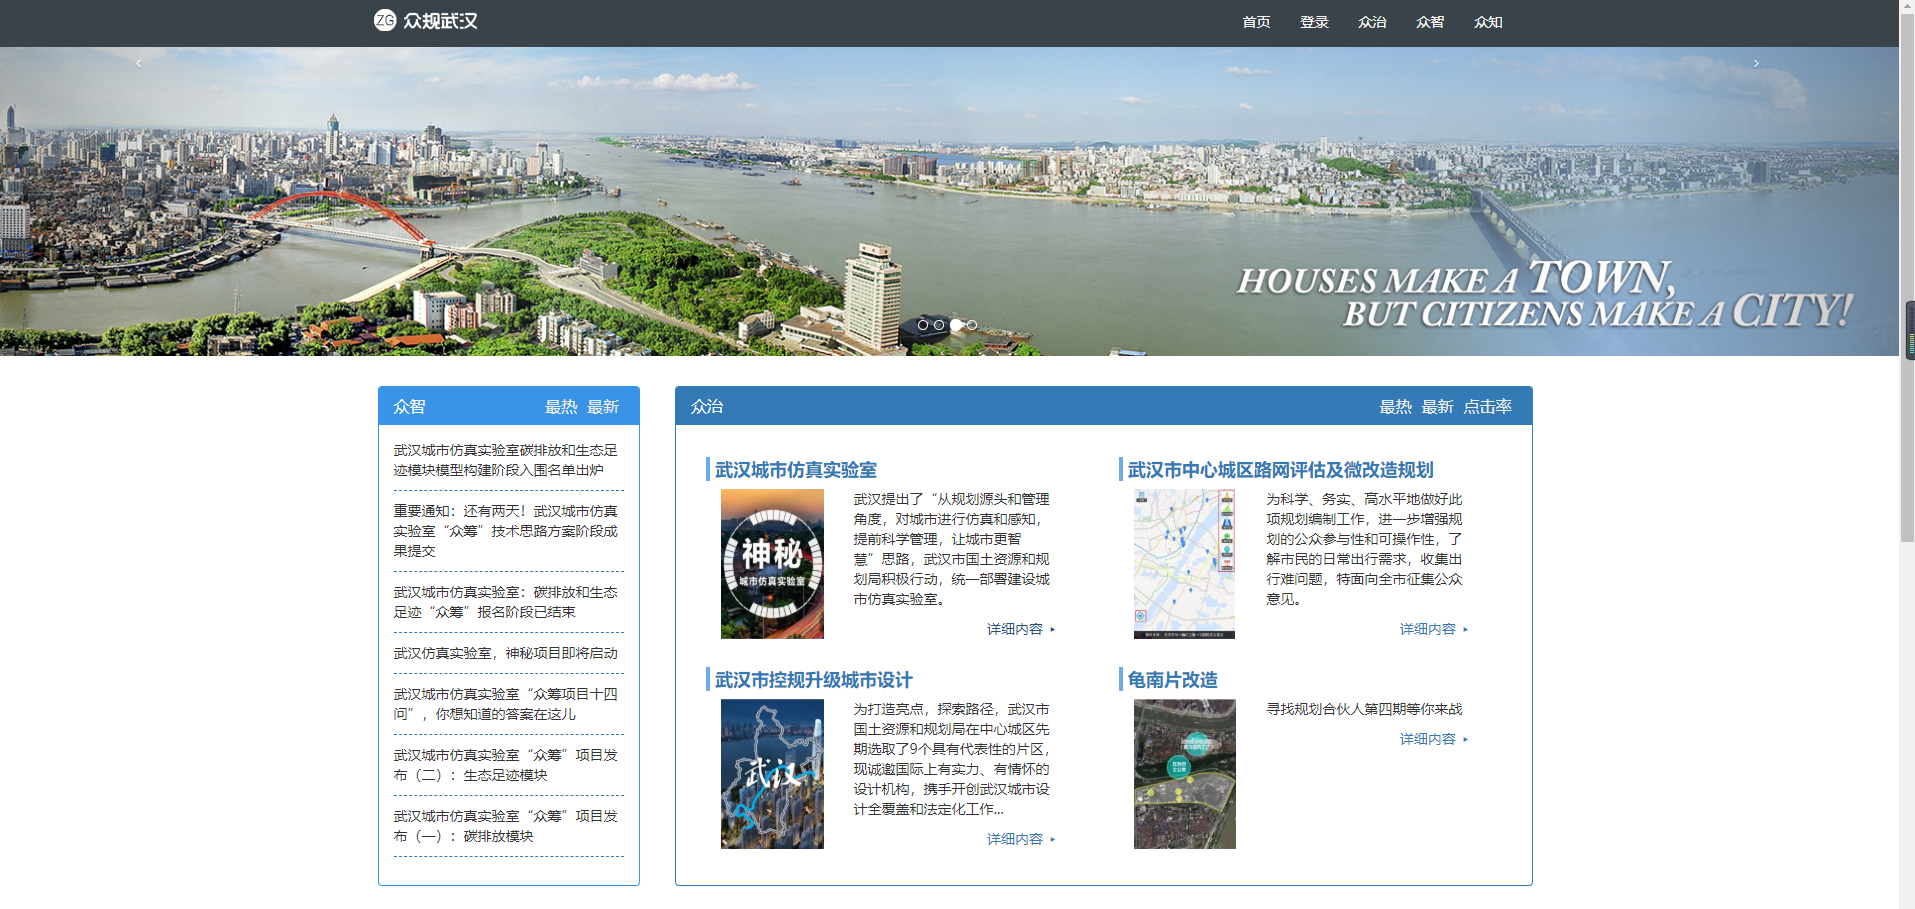
\includegraphics[width=0.85\textwidth]{chp05_武汉市众规平台.png}
  \caption{武汉市众规平台}
\end{figure}
  \end{onlyenv}

\vspace{-15pt}
  \begin{onlyenv}<2>
\begin{figure}
  \centering
  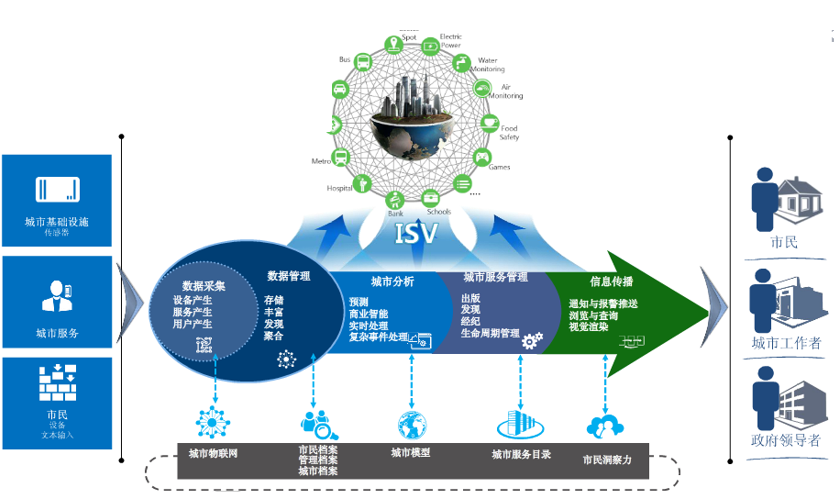
\includegraphics[width=0.7\textwidth]{chp05_政府共享平台.png}
  \caption{微软提出的基于大数据平台建设公共参与系统架构}
\end{figure}
  \end{onlyenv}
\end{overlayarea}
\end{frame}

\begin{frame}[t]{国家智慧城市建设战略的基础}
\begin{itemize}
\item<1-> 智慧城市建设已经成为国家战略
\begin{enumerate}
\item 《中共中央关于制定国民经济和社会发展第十三个五年规划的建议》
\item 国务院关于印发促进大数据发展行动纲要的通知
\item 《国家新型城镇化规划(2014-2020年)》
\end{enumerate}
\end{itemize}

\begin{overlayarea}{\textwidth}{\textheight}
\vspace{5pt}
  \begin{onlyenv}<2->
\begin{badbox}{智慧城市建设目标} 
更加智慧地推进新型城镇化建设,实现城乡一体化发展;产业升级、社会治理、生态环境修复、民生改善和基础设施功能提升,是智慧城市建设的方向。
\end{badbox}
  \end{onlyenv}
\end{overlayarea}
\end{frame}

\begin{frame}[t]{国家智慧城市建设战略的基础}
\begin{itemize}
\item<1-> 越来越多的非传统规划企业借助国家智慧城市建设的契机介入规划行业
\item<5-> 越来越多的数据通过大数据技术可以被连通和使用,但同时也对交通规划行业未来的发展提出了新的挑战
\end{itemize}

\begin{overlayarea}{\textwidth}{\textheight}
\vspace{-10pt}
  \begin{onlyenv}<2>
\begin{figure}
  \centering
  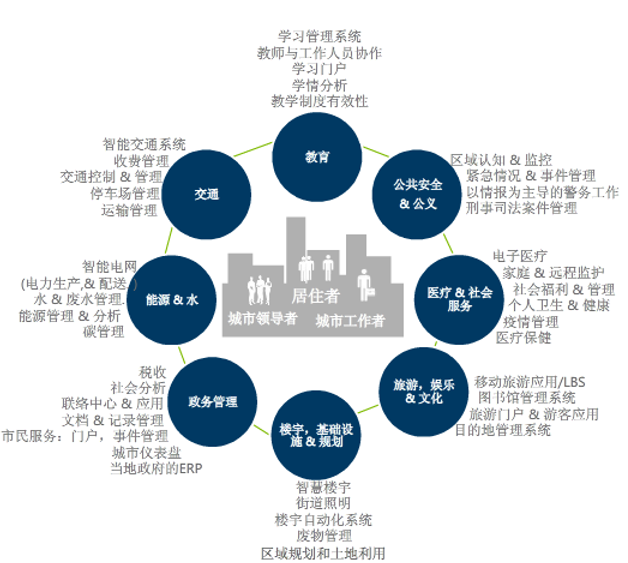
\includegraphics[width=0.55\textwidth]{chp05_微软智慧城市.png}
  \caption{微软公司的智慧城市建设解决方案}
\end{figure}
  \end{onlyenv}

  \begin{onlyenv}<3>
\begin{figure}
  \centering
  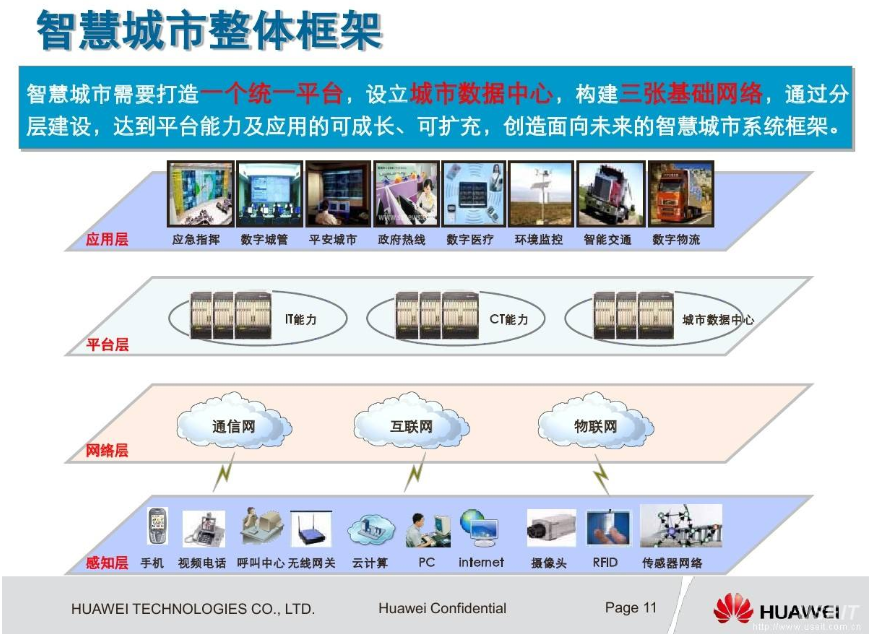
\includegraphics[width=0.65\textwidth]{chp05_华为智慧城市.png}
  \caption{华为公司的智慧城市建设解决方案}
\end{figure}
  \end{onlyenv}

  \begin{onlyenv}<4>
\begin{figure}
  \centering
  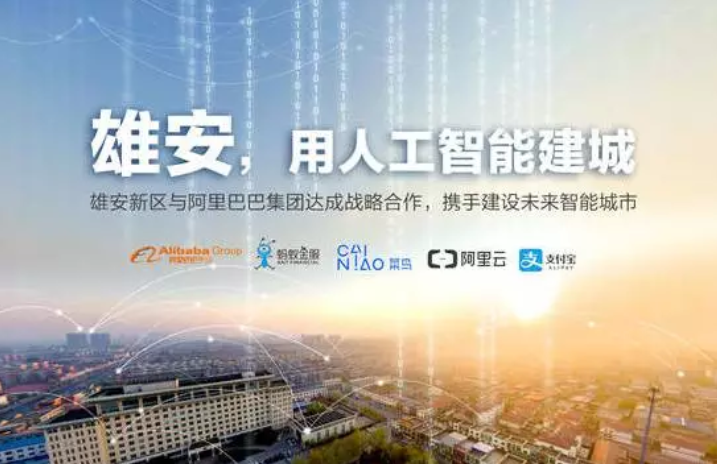
\includegraphics[width=0.7\textwidth]{chp05_阿里雄安.png}
  \caption{阿里巴巴参与雄安新区规划建设}
\end{figure}
  \end{onlyenv}
\end{overlayarea}
\end{frame}



